\documentclass[a4paper, 12pt]{article}%тип документа

%Русский язык
\usepackage[T2A]{fontenc} %кодировка
\usepackage[utf8]{inputenc} %кодировка исходного кода
\usepackage[english,russian]{babel} %локализация и переносы

%отступы 
\usepackage[left=2cm,right=2cm,top=2cm,bottom=3cm,bindingoffset=0cm]{geometry}

%Вставка картинок
\usepackage{graphicx}
\graphicspath{}
\DeclareGraphicsExtensions{.pdf,.png,.jpg, .jpeg}

%Таблицы
\usepackage[table,xcdraw]{xcolor}
\usepackage{booktabs}

%Графики
\usepackage{pgfplots}
\pgfplotsset{compat=1.9}

%Математика
\usepackage{amsmath, amsfonts, amssymb, amsthm, mathtools}

%Заголовок
\author{Подлесный Артём \\ группа 827}
\title{Работа 1.2.1 \\ Определение скорости полёта пули при помощи баллистического маятника}

\begin{document}
\maketitle

\paragraph{Цель работы:}
Определение скорости пули из пневматического ружья. Проверка закона сохранения массы.
\paragraph{Оборудование:}
Две установки с разными ружьями, наборы пуль, весы, подвешенный к потолку стальной груз, крутильная система со стальными грузами, оптические системы для определения отклонений грузов от положения равновесия, линейка. 
\section{Отчёт о работе}
\subsection{Массы пуль}

На таблице 1 представлены значения масс для всех пулек. Эксперимент проводила группа из трех нас, поэтому каждый из студентов проделывал все действия эксперимента со своим набором.

\begin{table}[]
\center
\caption{}
\begin{tabular}{|
>{\columncolor[HTML]{9B9B9B}}c |c|c|c|}
\hline
{\color[HTML]{333333} Пули} & \cellcolor[HTML]{9B9B9B}Белый набор, мг & \cellcolor[HTML]{9B9B9B}Тёмный набор, мг & \cellcolor[HTML]{9B9B9B}Третий набор, мг \\ \hline
{\color[HTML]{333333} 1}    & 503                               & 513                                & 517                           \\ \hline
{\color[HTML]{333333} 2}    & 508                               & 496                                & 517                           \\ \hline
{\color[HTML]{333333} 3}    & 514                               & 508                                & 510                           \\ \hline
{\color[HTML]{333333} 4}    & 507                               & 507                                & 499                           \\ \hline
{\color[HTML]{333333} 5}    & 512                               & 519                                & 516                           \\ \hline
{\color[HTML]{333333} 6}    & 517                               & 509                                & 514                           \\ \hline
{\color[HTML]{333333} 7}    & 501                               & 504                                & 504                           \\ \hline
{\color[HTML]{333333} 8}    & 509                               & 485                                & 508                           \\ \hline
\end{tabular}
\end{table}

\subsection{Метод баллистического маятника, совершающего поступательное движение.}

Измерения проводим на установке, указанной на рис.1.

\begin{figure}[h!]
\center{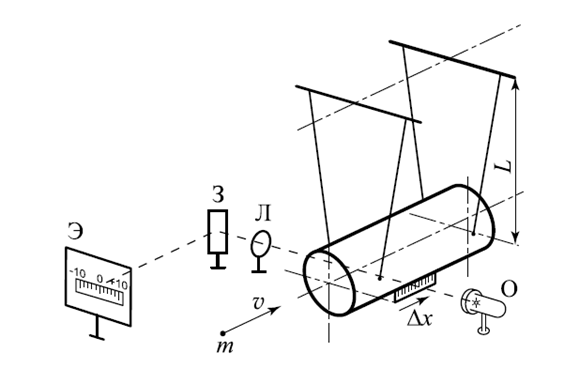
\includegraphics[scale=0.9]{f1.png}}
\caption{Математический маятник.}
\end{figure}

Во время самого первого выстрела внезапно отключилась лампа, поэтому нам пришлось обновить пулю, масса которой 519 мг. Далее она будет идти под номером 1 белого набора. В данной части эксперимента были использованы пули из белого набора и первые 4 пули из третьего набора. Кстати во втором эксперименте замерить отклонение маятника не удалось --- произошёл выход за границу шкалы. 

Высота нитей маятника --- $L=(224.7\pm2)\text{см}$.

Масса маятника --- $M=(2905\pm5)\text{ г}$.

При ударе о маятник сохраняется импульс. В предположении, что удар неупругий, то есть весь импульс пули передаётся маятнику, получаем, что:
\begin{equation}
u=\frac{M}{m}V,
\end{equation}

где V --- скорость маятника, u --- скорость пули. Здесь также использовано, что $m\ll M$. Кстати именно этим объясняется погрешность массы маятника. Пустой он весит $(2905\pm5)\text{ г}$, а с $\pm6$ пулями (среднее число пуль, лежащих внутри него) $(2908\pm8)\text{ г}$

В предположении, что отклонение маятника от вертикали мало (а это безусловно выполняется --- отклонения в несколько миллиметров при длине нити 2 м), используя ЗСЭ, получаем:
\begin{equation}
u=\frac{M}{m}\sqrt{\frac{g}{L}}\Delta x,
\end{equation}
где $\Delta x$ --- максимальное отклонение от вертикали в миллиметрах, измеряемая нами величина.

\begin{table}[]
\center
\caption{}
\begin{tabular}{|
>{\columncolor[HTML]{C0C0C0}}c |c|c|c|c|c|}
\hline
№ опыта & \cellcolor[HTML]{C0C0C0}$x_{0}$, мм & \cellcolor[HTML]{C0C0C0}$A_{0}$, мм & \cellcolor[HTML]{C0C0C0}$x_{max}$, мм & \cellcolor[HTML]{C0C0C0}$x_{end}$, мм & \cellcolor[HTML]{C0C0C0}$A_{end}$, мм \\ \hline
1       & -6                                  & 0,8                                 & 5,1                                   & -8,8                                  & 0,6                                   \\ \hline
3       & -2,5                                & 0,5                                 & 10                                    & -3                                    & 0,5                                   \\ \hline
4       & -3                                  & 0,5                                 & 9,5                                   & -7,3                                  & 0,25                                  \\ \hline
5       & -3                                  & 0,25                                & 9                                     & -3                                    & 1                                     \\ \hline
6       & -4                                  & 1                                   & 7,5                                   & -4                                    & 0,3                                   \\ \hline
7       & -3,3                                & 0,25                                & 9,3                                   & -3                                    & 0,3                                   \\ \hline
8       & -3,5                                & 0,5                                 & 6,5                                   & -5,3                                  & 1                                     \\ \hline
9       & -3,3                                & 0,5                                 & 7                                     & -4,7                                  & 0,3                                   \\ \hline
10      & -5                                  & 0,5                                 & 5                                     & -7                                    & 0,5                                   \\ \hline
11      & -2                                  & 0,2                                 & 8                                     & -3                                    & 0,4                                   \\ \hline
12      & -3,2                                & 0,4                                 & 3,8                                   & -6,2                                  & 0,3                                   \\ \hline
\end{tabular}
\end{table}

$x_{0}$ --- начальное значение на шкале.

$A_{0}$ --- амплитуда колебаний вокруг начального положения.

$x_{max}$ --- максимальное значение отклонения.

$x_{end}$ --- установившаяся координата после выстрела.

$A_{end}$ --- амплитуда колебаний вокруг конечного положения.

Исходя из этого мы можем получить скорости пуль, однако для чистоты проверим установку на добротность, что пренебрежение трением действительно оправдано. Для этого на исследуемом диапазоне проверим, на сколько затухают колебания. Из прошлой работы нам известно, что модель вязкого трения хоть и не оправдана теоретически, но практически хорошо приближает данные. Из этого мы сможем оценить на сколько может быть занижена максимальная амплитуда.

\begin{table}[]
\center
\caption{}
\begin{tabular}{|c|c|c|}
\hline
\begin{tabular}[c]{@{}c@{}}$A_{0}$,\\   мм\end{tabular} & $A_{10}$, мм & $A_{1}$, мм \\ \hline
3,8                                                     & 3,6          & 3,78        \\ \hline
\end{tabular}
\end{table}
%здесь должна быть проверка

Получается, что влиянием трения действительно можно пренебречь.
Так как сама установка смещалась во время выстрела, то можно посчитать скорость пули исходя из двух моделей: время взаимодействия ружья со столом много меньше, чем время полёта пули и наоборот. Эти скорости можно посчитать по формуле (2). Получившиеся оценки обозначим $u_0$ и $u_{end}$. Погрешности, как уже говорилось случайные, поэтому погрешности оцениваем по "правилу трёх сигм".

\[u_{0}=(129\pm20\text{ м/с.})\]

\[u_{end}=(147\pm21)\text{ м/с.}\]


\subsection{Метод крутильного баллистического маятника.}
Измерения проводим на установке, указанной на рис.2.

\begin{figure}[h!]
\center{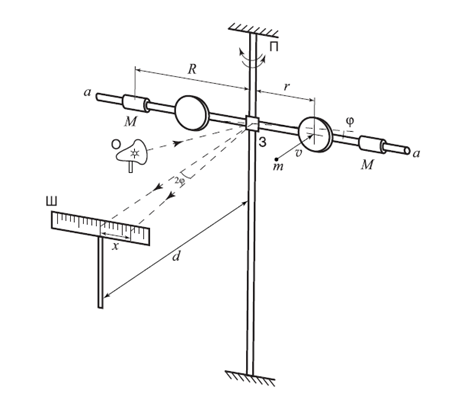
\includegraphics[scale=0.9]{f2.png}}
\caption{Математический маятник.}
\end{figure}

В данной части работы мы будем стрелять в одну из "болванок", расстояние до которых от оси вращения 8,5 см. Будут использоваться все оставшиеся пули, кроме двух последних из третьего набора. Опять же в предположении неупругого удара получаем, что момент импульса сохраняется. Запишем это, учитывая, что массой пуль после удара можно пренебречь:

\[mur=I\Omega,\]
где $\Omega$ --- начальная угловая скорость вращения после удара.

При отклонении маятника на небольшой угол от равновесного положения возникает возвращающая сила, в первом приближении пропорциональная углу отклонения. Коэффициент пропорциональности обозначим $k$. Тогда:

\[k\frac{\phi^2}{2}=I\frac{\Omega^2}{2},\]
где $\phi$ --- максимальный угол отклонения. Получается:

\[u=\phi\frac{\sqrt{kI}}{mr}\]

Для определения максимального угла отклонения будем использовать шкалу и лампочку, светящую на отражающую поверхность маятника. Из рисунка 3 следует:

\[\phi\approx\frac{x}{2d}\]

Для установления связи "непонятного" $kI$ с нашим экспериментом, измерим периоды вращения маятника с грузами и без них. Принципиальное отличие этих экспериментов в том, что момент инерции во втором случае меньше.

\[T_{1}=2\pi\sqrt{\frac{I}{k}}\]

\[T_{2}=2\pi\sqrt{\frac{I-(M_{1}+M_{2})}{k}}\]

$M_1$ и $M_2$ --- массы съёмных грузов.

\[\sqrt{kI}=\frac{2\pi(M_1+M_2)R^2T_1}{T^2_1-T^2_2}\]

Используя изложенные выше формулы получаем:
\begin{equation}
u=\frac{\pi x(M_1+M_2)R^2T_1}{mrd(T^2_1-T^2_2)}.
\end{equation}

Параметры установки приведены в таблице 4. Различные значения d - в начале и в конце эксперимента.

\begin{table}[]
\center
\caption{}
\begin{tabular}{|
>{\columncolor[HTML]{C0C0C0}}c |c|}
\hline
r, см     & 18   \\ \hline
R, см     & 28,5  \\ \hline
$d_0$, см & 34    \\ \hline
d, см     & 36    \\ \hline
$M_1$, г  & 729,6 \\ \hline
$M_2$, г  & 729,9 \\ \hline
$T_2$, с  & 8,24  \\ \hline
$T_1$, с  & 10,88 \\ \hline
\end{tabular}
\end{table}

\begin{table}[]
\center
\caption{}
\begin{tabular}{|
>{\columncolor[HTML]{9B9B9B}}c |c|c|c|c|c|c|}
\hline
№ опыта & \cellcolor[HTML]{9B9B9B}$x_{0}$, cм & \cellcolor[HTML]{9B9B9B}$A_{0}$, мм & \cellcolor[HTML]{9B9B9B}$x_{max}$, cм & \cellcolor[HTML]{9B9B9B}$x_{end}$, cм & \cellcolor[HTML]{9B9B9B}$A_{end}$, cм & \cellcolor[HTML]{9B9B9B}$m$, мг \\ \hline
1       & 0,5                                 & 0,5                                 & 5,2                                   & 0                                     & 0,5                                   & 513                             \\ \hline
2       & 0,3                                 & 0,8                                 & 6,3                                   & 0,5                                   & 0,5                                   & 496                             \\ \hline
3       & 0                                   & 0,5                                 & 5                                     & 0                                     & 1                                     & 508                             \\ \hline
4       & 0                                   & 1                                   & 5,5                                   & 0                                     & 0,2                                   & 507                             \\ \hline
5       & 0                                   & 0,5                                 & 5,8                                   & -0,3                                  & 0,3                                   & 519                             \\ \hline
6       & -0,3                                & 0,5                                 & 6                                     & -0,1                                  & 0,6                                   & 509                             \\ \hline
7       & -0,5                                & 0,5                                 & 5,1                                   & -0,5                                  & 0,1                                   & 504                             \\ \hline
8       & -0,5                                & 0,5                                 & 4,9                                   & -0,5                                  & 0,5                                   & 485                             \\ \hline
9       & -0,6                                & 0,5                                 & 5                                     & -0,8                                  & 0,3                                   & 516                             \\ \hline
10      & -0,5                                & 0,2                                 & 5,4                                   & -0,5                                  & 0,5                                   & 514                             \\ \hline
\end{tabular}
\end{table}

Как и в прошлом эксперименте, трением можно пренебречь. За 10 колебаний амплитуда снизилась с 5.4 см до 4.6 см, а значит за одно колебание амплитуда уменьшилась примерно на 1 мм, что примерно в 5 раз меньше даже амплитуды колебаний вокруг начального положения.

В итоге, сталкиваясь с аналогичной проблемой, как и в прошлом пункте, мы понимаем, что можно привести две оценки значения скорости. Кстати из-за того, что в конечной формуле стоит много косвенно измеренных величин, погрешность периодов может достигать 0.1 с, пренебрегать систематической погрешностью нельзя, ведь она примерно 12\%. 

\[u'_{0}=(140\pm21)\text{ м/с.}\]

\[u'_{end}=(142\pm19)\text{ м/с.}\]


\section{Вывод}
Мы показали, что используя баллистические маятники, З.С.И и З.С.Э. можно вычислить скорость мелких быстролетящих объектов.
 
Мы измерили скорость пули, вылетающей из духового ружья. Сильное отклонение $u_{0}$ от остальных можно объяснить тем, что "скачок" стола происходил достаточно быстро, а в крутильном маятнике "скачок" был мал. В силу сильного отклонения доверять этому значению не надо. Причиной этому можно указать, что, наверно, ружья могли стрелять под некоторым углом к поверхности соприкосновения. 

В каждом из экспериментов мы получили две оценки скорости. Они не сильно отличаются, так что для конечного ответа мы можем брать любое из них. Взяв среднее, получаем:

\[u=(143\pm12)\text{ м/с.}\]
\end{document}
